\chapter{Algorithms}
\label{sec:algorithms}

Now that we have defined episodes and association rules on sequences, and their respective measures of frequency and confidence, we are ready to present algorithms that find all frequent episodes and confident association rules. We won't repeat the definitions, but it is useful to keep them in mind, in order to see exactly how the algorithms accomplish their task.

We will start with the algorithms that find episodes, and then move on to association rules. For each, we'll gove a sketch of the full procedure outlining the high-level steps, before drilling down into the details.

\section{Finding frequent episodes: high-level algorithm}

\begin{algorithm}

\caption{High-level algorithm for finding frequent episodes. \\
Input: A set $ \Sigma $ of event types, an episode class~$ \mathcal{E} $ (parallel or serial), a frequency measure~$ \Psi $ an event sequence $ \boldsymbol{s} $ over $ \Sigma $, a window width $ \rho $, and a frequency threshold \emph{min\_fr}. \\
Output: The collection of episodes that are frequent in the sequence in terms of the input parameters.
}

\begin{algorithmic}[1]

\State $ \mathcal{C}_1 \gets \{ \langle A \rangle \mid A \in \Sigma \} $
\State $ l \gets 1 $
\While{$ \mathcal{C}_l \neq \emptyset $}
    \LineComment{Database pass (different subalgorithms depending on $ \mathcal{E} $)}
    \State compute $ \mathcal{F}_l \gets \{ \alpha \in \mathcal{C}_l \mid fr_\Psi(\alpha, \boldsymbol{s}, \rho) \geq \text{min\_fr} \} $
    \State $ l \gets l + 1 $
    \LineComment{Candidate generation (algorithm \ref{alg:cand-gen})}
    \State compute $ \mathcal{C}_l = \{ \alpha \mid | \alpha | = l \wedge \forall \beta \mid \beta \subset \alpha : fr_\Psi(\beta, \boldsymbol{s}, \rho) \geq \text{min\_fr} \} $
\EndWhile
\State output all $ \mathcal{F}_i $

\end{algorithmic}

\label{alg:episodes-top-level}
\end{algorithm}

% TODO Read this future me, probably needs improvement.

Algorithm~\ref{alg:episodes-top-level} (adapted from~\citep{mannila1997discovery}) describes the high-level procedure to find all frequent episodes of a given class of episodes---parallel or serial---that are frequent in an event sequence $ \boldsymbol{s} $, given window width $ \rho $ and frequency threshold \emph{min\_fr}. It is a breadth-first algorithm, that is, all frequent episodes of size $ l $ are computed before those of size $ l + 1 $. The algorithm finds either parallel or serial episodes, not both simultaneously, since both require different subalgorithms, except for episodes which contain only one event type; those are equivalent to each other. Of course the chosen frequency measure also influences the output.

The construction of the first set of candidates is a special case. $ \mathcal{C}_1 $ consists of simply all possible episodes with one node. That's one episode per event type, and so $ | C_1 | = | \Sigma | $. After constructing $ \mathcal{C}_1 $ a loop is entered where ever-bigger episodes are constructed and then filtered by frequency in the sequence.
% for each $ l $, it is determined which episodes are frequent ($ \mathcal{F}_1 $), by a pass over the sequence, and subsequently, based on those, candidates of size $ 2 $ are generated. The loop continues with ever-increasing episode size $ l $, and stops when no more candidates were generated. Then all frequent episodes have been found.

The following subsections will cover all of the subalgorithms. Candidate generation is identical for all frequency measures---with only a slight variation between parallel and serial episodes (algorithm~\ref{alg:cand-gen}, section~\ref{sec:cand-gen}). Determining which of the candidates are frequent, is more involved and highly depends on both the episode class and the frequency measure (algorithms~\ref{alg:rec-par-fwi} through \ref{alg:remove-infrequent-episodes}, sections~\ref{sec:rec-par-fwi} through \ref{sec:maintain-blocks}).

\section{Candidate generation}
\label{sec:cand-gen}

\begin{algorithm}

\caption{Generating candidate parallel episodes of size $ l + 1 $ from frequent parallel episodes of size $ l $. \\
Input: A sorted array $ \mathcal{F}_l $ of frequent parallel episodes of size $ l $. \\
Output: A sorted array of candidate parallel episodes of size $ l + 1 $.
}

\begin{algorithmic}[1]

\State $ \mathcal{C}_{l + 1} \gets \text{empty array} $
\State $ k \gets 0 $
\If{$ l = 1 $}
    \For{$ h \gets 1 $ to $ | \mathcal{F}_l | $} $ \mathcal{F}_l \text{.block\_start}[h] \gets 1 $ \EndFor
\EndIf
\For{$ i \gets 1 $ to $ | \mathcal{F}_l | $} \label{alglin:cand-gen:i-loop}
    \State $ \text{current\_block\_start} \gets k + 1 $
    \For{$ j \gets i $; $ \mathcal{F}_l \text{.block\_start}[j] = \mathcal{F}_l \text{.block\_start}[i] $; $ j \gets j + 1 $}
    \label{alglin:cand-gen:j-loop}
        \LineComment{$ \mathcal{F}_l[i] $ and $ \mathcal{F}_l[j] $ have $ l - 1 $ first event types in common, build a potential candidate $ \alpha $ as their combination.}
        \For{$ x \gets 1 $ to $ l $} $ \alpha[x] \gets \mathcal{F}_l[i][x] $ \label{alglin:cand-gen:construct-candidate-1}
        \EndFor
        \State $ \alpha[l + 1] \gets \mathcal{F}_l[j][l] $ \label{alglin:cand-gen:construct-candidate-2}
        \LineComment{Build and test subepisodes $ \beta $ that do not contain $ \alpha[y] $}
        \For{$ y \gets 1 $ to $ l - 1 $} \label{alglin:cand-gen:test-subepisodes-loop}
            \For{$ x \gets 1 $ to $ y - 1 $} $ \beta[x] \gets \alpha[y] $
            \EndFor
            \For{$ x \gets y $ to $ l $} $ \beta[x] \gets \alpha[x + 1] $
            \EndFor
            \If{$ \beta $ is not in $ \mathcal{F}_l} $ continue with the next $ j $ at line~\ref{alglin:cand-gen:j-loop}
            \EndIf
        \EndFor
        \LineComment{All subepisodes are in $ \mathcal{F}_l $, store $ \alpha $ as candidate}
        \State $ k \gets k + 1 $
        \State $ \mathcal{C}_{l + 1}[k] \gets \alpha $
        \State $ \mathcal{C}_{l + 1} \text{.block\_start}[k] \gets \text{current\_block\_start} $
    \EndFor
\EndFor
\State output $ \mathcal{C}_{l + 1} $

\end{algorithmic}

\label{alg:cand-gen}
\end{algorithm}

Algorithm~\ref{alg:cand-gen} (from~\citep{mannila1997discovery}) generates candidates of size $ l + 1 $ from a collection of frequent parallel episodes of size $ l $. It can be easily modified to generate serial episodes, as we'll show later in this subsection. Thanks to the monotonic property of the frequency measures we implement, some candidates can be immediately proven infrequent. More specifically, if there exists an infrequent subepisode $ \beta $ of candidate $ \alpha $, then $ \alpha $ is not frequent.
Conveniently, all frequent subepisodes of size $ l $ are already given as input to the algorithm. So when the algorithm constructs a candidate of size $ l + 1 $, all of its subepisodes of size $ l $ are checked to be frequent by testing whether they are in the input collection $ \mathcal{F}_l $. If one of the subepisodes is not in $ \mathcal{F}_l $, then it is infrequent and, consequently, the potential candidate cannot be frequent either.
Subepisodes smaller than $ l $ do not need to be checked anymore, because any less-than-$ l $-sized subepisode of the potential candidate is also a subepisode of one of the $ l $-sized subepisodes and any $ l $-sized subepisodes that have turned out to be frequent are already known to have frequent subepisodes.

% Combine this paragraph with the one about parallel episode candidate generation?
Parallel episodes are constructed such that the elements in their arrays are sorted according to event type. In this way, a parallel episode has a unique array representation.

Potential candidates of size $ l + 1 $ are generated by combining frequent episodes of size $ l $ which share a prefix of $ l - 1 $ elements. In other words, they are only allowed to differ in their last element. The newly constructed candidate shares these $ l - 1 $ as well, and is then followed by the last elements of both $ \alpha $ and $ \beta $. This method of candidate generation is similar to the way in which candidate itemsets are generated in the Apriori algorithm \citep{mannila1997discovery}. Lines~\ref{alglin:cand-gen:construct-candidate-1} and \ref{alglin:cand-gen:construct-candidate-2} implement this. Figure~\ref{fig:parallel-episode-combined} shows an example of two episodes being combined, and figure~\ref{fig:parallel-episode-lattice} shows visually how larger candidates build upon smaller episodes.

\begin{figure}
\centering

\begin{tikzpicture}

\newcommand\sharedprefix[1]
{
    \ifcase#1 a
    \or a
    \or b
    \fi
}

\foreach \arrayindex [evaluate=\arrayindex as \leftx using int(\arrayindex-4),
                      evaluate=\arrayindex as \rightx using (int(\arrayindex+1))] in {0,...,2}
{
    \node (n\arrayindex0) [arraycell,enoughdamnvspace] at (\leftx,0.75) {$ \sharedprefix{\arrayindex} $};
    \node (n\arrayindex1) [arraycell,enoughdamnvspace] at (\leftx,-0.75) {$ \sharedprefix{\arrayindex} $};
    \node (n\arrayindex2) [arraycell,enoughdamnvspace] at (\rightx,0) {$ \sharedprefix{\arrayindex} $};
}

\node (n30) [arraycell,enoughdamnvspace,color=red!90!black] at (-1,0.75) {$ b $};
\node (n31) [arraycell,enoughdamnvspace,color=blue!90!black] at (-1,-0.75) {$ c $};

\node (n32) [arraycell,enoughdamnvspace,color=red!90!black] at (4,0) {$ b $};
\node (n42) [arraycell,enoughdamnvspace,color=blue!90!black] at (5,0) {$ c $};

\draw [->] (n30.north) to [bend left=45] (n32.north);
\draw [->] (n31.south) to [bend right=45] (n42.south);

\draw [accolade] (n21.south east) -- node (acc1tip) [inner sep=0,midway,yshift=-10pt] {} (n01.south west);
\draw [accolade] (n22.south east) -- node (acc2tip) [inner sep=0,midway,below,yshift=-10pt] {} (n02.south west);

\draw [->] (acc1tip) to [bend right=45] (acc2tip);

% \node [above=of n00] {first episode};
% \node [below=of n01] {second episode};

\node [right=5pt of n42] {potential candidate};

\end{tikzpicture}

\caption{Two episodes with a shared prefix being combined into a larger episode.}
\label{fig:parallel-episode-combined}
\end{figure}

\begin{figure}
\centering

\begin{tikzpicture}

\node (e) at (0,0) {$ \emptyset $};

\iffalse % without braces, commas
\node [enoughdamnvspace] (A) at (-1,-1) {$ a $};
\node [enoughdamnvspace] (B) at (0,-1) {$ b $};
\node [enoughdamnvspace] (C) at (1, -1) {$ c $};

\node [enoughdamnvspace] (AA) at (-2.5,-2) {$ aa $};
\node [enoughdamnvspace] (AB) at (-1.5,-2) {$ ab $};
\node [enoughdamnvspace] (AC) at (-0.5,-2) {$ ac $};
\node [enoughdamnvspace] (BB) at (0.5,-2) {$ bb $};
\node [enoughdamnvspace] (BC) at (1.5,-2) {$ bc $};
\node [enoughdamnvspace] (CC) at (2.5,-2) {$ cc $};

\node [enoughdamnvspace] (AAA) at (-6,-3.5) {$ aaa $};
\node [enoughdamnvspace] (AAB) at (-4.5,-3.5) {$ aab $};
\node [enoughdamnvspace] (AAC) at (-3,-3.5) {$ aac $};
\node [enoughdamnvspace] (ABB) at (-1.5,-3.5) {$ abb $};
\node [enoughdamnvspace] (ABC) at (0,-3.5) {$ abc $};
\node [enoughdamnvspace] (BBB) at (1.5,-3.5) {$ bbb $};
\node [enoughdamnvspace] (BBC) at (3,-3.5) {$ bbc $};
\node [enoughdamnvspace] (BCC) at (4.5,-3.5) {$ bcc $};
\node [enoughdamnvspace] (CCC) at (6,-3.5) {$ ccc $};
\fi

% with braces, commas
\node [enoughdamnvspace] (A) at (-1,-1) {$ \{ a \} $};
\node [enoughdamnvspace] (B) at (0,-1) {$ \{ b \} $};
\node [enoughdamnvspace] (C) at (1, -1) {$ \{ c \} $};

\node [enoughdamnvspace] (AA) at (-2.5,-2) {$ \{ a, a \} $};
\node [enoughdamnvspace] (AB) at (-1.5,-2) {$ \{ a, b \} $};
\node [enoughdamnvspace] (AC) at (-0.5,-2) {$ \{ a, c \} $};
\node [enoughdamnvspace] (BB) at (0.5,-2) {$ \{ b, b \} $};
\node [enoughdamnvspace] (BC) at (1.5,-2) {$ \{ b, c \} $};
\node [enoughdamnvspace] (CC) at (2.5,-2) {$ \{ c, c \} $};

\node [enoughdamnvspace] (AAA) at (-6,-3.5) {$ \{ a, a, a \} $};
\node [enoughdamnvspace] (AAB) at (-4.5,-3.5) {$ \{ a, a, b \} $};
\node [enoughdamnvspace] (AAC) at (-3,-3.5) {$ \{ a, a, c \} $};
\node [enoughdamnvspace] (ABB) at (-1.5,-3.5) {$ \{ a, b, b \} $};
\node [enoughdamnvspace] (ABC) at (0,-3.5) {$ \{ a, b, c \} $};
\node [enoughdamnvspace] (BBB) at (1.5,-3.5) {$ \{ b, b, b \} $};
\node [enoughdamnvspace] (BBC) at (3,-3.5) {$ \{ b, b, c \} $};
\node [enoughdamnvspace] (BCC) at (4.5,-3.5) {$ \{ b, c, c \} $};
\node [enoughdamnvspace] (CCC) at (6,-3.5) {$ \{ c, c, c \} $};

\draw (e) -- (A);
\draw (e) -- (B);
\draw (e) -- (C);

\draw (A) -- (AA);
\draw (A) -- (AB);
\draw (B) -- (AB);
\draw (A) -- (AC);
\draw (C) -- (AC);
\draw (B) -- (BB);
\draw (B) -- (BC);
\draw (C) -- (BC);
\draw (C) -- (CC);

\draw (AA) -- (AAA);
\draw (AA) -- (AAB);
\draw (AB) -- (AAB);
\draw (AB) -- (ABB);
\draw (AA) -- (AAC);
\draw (AC) -- (AAC);
\draw (AB) -- (ABC);
\draw (AC) -- (ABC);
\draw (BB) -- (BBB);
\draw (BB) -- (BBC);
\draw (BC) -- (BBC);
\draw (BC) -- (BCC);
\draw (CC) -- (BCC);
\draw (CC) -- (CCC);

\end{tikzpicture}

\caption{Parallel episode construction for $ \Sigma = \{ a, b, c \} $ up to size 3.}

\label{fig:parallel-episode-lattice}
\end{figure}

The algorithm assumes that the input array of frequent $ l $-sized episodes $ \mathcal{F}_l $ is sorted lexicographically. That is, the episodes are firstly sorted by the first event type in their array representation; those episodes which share their first element are sorted by the second element, and so on. Therefore episodes which share a prefix are grouped together. The algorithm constructs new episodes in such a way that the output is also ordered lexicographically, and since part of the output of one run becomes the input of the next, the assumption about the input is always true.

As mentioned previously, a potential candidate is generated from two episodes that share an $ (l - 1) $-prefix in their array representation. And with the episodes being ordered as described, all of the episodes that share a prefix are grouped together. As a result, episodes can be grouped into \emph{blocks}, where all of the episodes in a block share the first $ l - 1 $ elements. All episodes within the same block are combined. Figure~\ref{fig:blocks} illustrates the block structure.

\newcommand\blockspicvalue[2]{
    \ifcase#2
        \ifcase#1 a
            \or a
            \or b
        \fi
        \or \ifcase#1 a
            \or a
            \or c
        \fi
        \or \ifcase#1 a
            \or c
            \or c
        \fi
        \or \ifcase#1 a
            \or c
            \or d
        \fi
        \or b
        \or \ifcase#1 b
            \or b
            \or c
        \fi
        \or \ifcase#1 b
            \or b
            \or d
        \fi
        \or c
    \fi
}

\begin{figure}
\centering

\begin{tikzpicture}

\foreach \x in {0,...,2}
\foreach \y in {0,...,7}
{
    \node (n\x\y) [draw,enoughdamnvspace,minimum size=1cm] at (\x,-\y*1.1) {$ \blockspicvalue{\x}{\y} $};
}

\draw [accolade] ([yshift=2pt]n00.north west) -- ([yshift=2pt]n10.north east) node [midway,above=12pt] {episodes with shared 2-prefix form a block};

\draw [accolade] ([xshift=2pt]n20.north east) -- ([xshift=2pt]n21.south east) node [midway,right=12pt] {block};
\draw [accolade] ([xshift=2pt]n22.north east) -- ([xshift=2pt]n23.south east) node [midway,right=12pt] {block};
\draw [accolade] ([xshift=2pt]n24.north east) -- ([xshift=2pt]n26.south east) node [midway,right=12pt] {block};
\draw [decorate,decoration={brace,amplitude=5pt}] ([xshift=2pt]n27.north east) -- ([xshift=2pt]n27.south east) node [midway,right=12pt] {block};

\end{tikzpicture}

\caption{Blocks in candidate generation algorithm with parallel episodes of size 3.}

\label{fig:blocks}
\end{figure}

The block structure is represented as follows.
Each episode $ \alpha $ is associated with a value \emph{block\_start}, which is the array index of the first episode in the block which contains $ \alpha $, so it points ``back'' to the beginning of the block. The first episode in each block points to itself. In this way, it can be easily tested whether two episodes belong to the same block. Figure~\ref{fig:block-values} shows this representation for the episodes in figure~\ref{fig:blocks}.

\begin{figure}
\centering

\begin{tikzpicture}

\newcommand\blockspicvaluevalue[1]
{
    \ifcase#1 1
    \or 1
    \or 3
    \or 3
    \fi
}

\foreach \y [evaluate=\y as \arrayindex using int(\y+1)] in {0,...,3}
{
    \foreach \x in {0,...,2}
    {
        \node (n\x\y) [draw,enoughdamnvspace,minimum size=1cm] at (\x,-\y*1.1) {$ \blockspicvalue{\x}{\y} $};
    }
    \node [left=10pt of n0\y] {$ \arrayindex $};
    \node [right=10pt of n2\y] {$ \blockspicvaluevalue{\y} $};
}

\node [above left=0 of n00] {array index};
\node [above right=0 of n20] {block\_value};
\node [below=0 of n13] {$ \vdots $};

\end{tikzpicture}

\caption{How blocks are represented in the candidate generation algorithm.}
\label{fig:block-values}
\end{figure}

The algorithm constructs this block structure while generating candidates of size $ l + 1 $, but it also uses the blocks of the $ l $-sized episodes given as input. So it is important that they are preserved and maintained in between different runs of algorithm~\ref{alg:cand-gen}. Section~\ref{sec:maintain-blocks} goes into more detail about this.

We mentioned earlier that in the array representation of parallel episodes, elements are sorted according to event type. We would like to construct parallel candidates for which this is the case as well. We know that the input array of frequent episodes is sorted, and that all episodes in a block share an $ (l - 1) $-prefix. Consequently, for any two episodes $ \mathcal{C}[i] $ and $ \mathcal{F}[j] $ in a block such that $ i \leq j $, it holds that $ \mathcal{F}[i][l] \leq \mathcal{F}[j][l] $.
Now, if we always construct a new candidate $ \alpha $ as $ \langle \mathcal{F}[i][1], \ldots,\allowbreak\mathcal{F}[i][l],\allowbreak\mathcal{F}[j][l] \rangle $ and choose $ i $ and $ j $ such that $ i \leq j $, then $ \alpha $'s array representation is sorted by construction. This explains the nested-loop structure of the algorithm (lines~\ref{alglin:cand-gen:i-loop} and~\ref{alglin:cand-gen:j-loop}), where the inner array index $ j $ is always greater than or equal to the outer index $ i $.

With serial episodes on the other hand, the order of elements in the array is not bound by an order on the event types.
Serial candidate generation can be accomplished by a small change to the algorithm. Line~\ref{alglin:cand-gen:j-loop} needs to be changed to:
\begin{algorithmic}[0]
\For{$ j \gets \mathcal{F}_l. \text{block\_start}[i] $; $ \mathcal{F}_l \text{.block\_start}[j] = \mathcal{F}_l \text{.block\_start}[i] $; $ j \gets j + 1 $}
\EndFor
\end{algorithmic}
By initializing $ j $ to $ \mathcal{F}_l \text{.block\_start}[i] $, $ j $ can be less than $ i $, and candidates $ \alpha $ with have $ \alpha[l] > \alpha[l + 1] $ will be generated, alleviating the constraint on parallel episodes.

Given the fact that $ \mathcal{F}_l $ is sorted lexicographically, and because of the order in which the algorithm traverses $ \mathcal{F}_l $, it is easy to see that the output array $ \mathcal{C}_{l + 1} $ of candidates will be sorted lexicographically as well.

After constructing a potential candidate (lines~\ref{alglin:cand-gen:construct-candidate-1} and \ref{alglin:cand-gen:construct-candidate-2}), it needs to be checked whether all of its subepisodes are frequent.
Constructing all $ l $-sized subepisodes of an $ (l + 1) $-sized candidate $ \alpha $ is straightforward. For each subepisode, one node from $ \alpha $'s graph is left out, until all nodes have been left out. For serial episodes, the edges of the subepisode are constructed such that the order of the toplogical sort is preserved.
% If we consider the strict form of a serial candidate, an $ l $-sized subepisode can be obtained by leaving one node $ v $ and all edges that contain $ v $.
For the array representation of both classes of episodes, this means that one element of the array is left out. See figure~\ref{fig:cand-subepisodes} for an example. In the algorithm, this happens at lines~\ref{alglin:cand-gen:test-subepisodes-loop} and further. The variable $ y $ denotes the array index of the element that will be left out.

For any potential candidate, two subepisodes in particular are already known to be frequent, namely the episodes it was built from. Those subepisodes are obtained by leaving out the last and the second to last array elements, respectively. That's why $ l - 1 $ is the largest value that $ y $ takes in the algorithm.

We should note that in the subepisode construction procedure described above, some of the subepisodes may be equivalent to each other, when an event type occurs multiple times in a candidate. For candidate $ \{ a, a, b \} $, subepisode $ \{ a, b \} $ will be constructed twice.

\begin{figure}
\centering

\begin{tikzpicture}

\node at (2,1) {potential 4-candidate};
\node at (6,2.65) {3-subepisodes};

\node [arraycell,enoughdamnvspace] at (0.5,0) {$ a $};
\node [arraycell,enoughdamnvspace] at (1.5,0) {$ b $};
\node [arraycell,enoughdamnvspace] at (2.5,0) {$ c $};
\node [arraycell,enoughdamnvspace] at (3.5,0) {$ d $};

\node [arraycell,enoughdamnvspace] at (5,1.65) {$ b $};
\node [arraycell,enoughdamnvspace] at (6,1.65) {$ c $};
\node (r0) [arraycell,enoughdamnvspace] at (7,1.65) {$ d $};
\node [right=10pt of r0] {drop $ a $};
\draw [red,very thick] (4.5,2.15) -- ++(0,-1);

\node [arraycell,enoughdamnvspace] at (5,0.55) {$ a $};
\node [arraycell,enoughdamnvspace] at (6,0.55) {$ c $};
\node (r1) [arraycell,enoughdamnvspace] at (7,0.55) {$ d $};
\node [right=10pt of r1] {drop $ b $};
\draw [red,very thick] (5.5,1.05) -- ++(0,-1);

\node [arraycell,enoughdamnvspace] at (5,-0.55) {$ a $};
\node [arraycell,enoughdamnvspace] at (6,-0.55) {$ b $};
\node (r2) [arraycell,enoughdamnvspace] at (7,-0.55) {$ d $};
\node (dropC) [right=10pt of r2] {drop $ c $};
\draw [red,very thick] (6.5,-0.05) -- ++(0,-1);

\node [arraycell,enoughdamnvspace] at (5,-1.65) {$ a $};
\node [arraycell,enoughdamnvspace] at (6,-1.65) {$ b $};
\node (r3) [arraycell,enoughdamnvspace] at (7,-1.65) {$ c $};
\node (dropD) [right=10pt of r3] {drop $ d $};
\draw [red,very thick] (7.5,-1.15) -- ++(0,-1);

\draw [accolade] (dropC.east |- r2.north) -- node [midway,right,align=left,xshift=10pt] {last two are frequent\\since candidate was\\built upon them} (dropD.east |- r3.south);

\end{tikzpicture}

\caption{The construction of $ l $-sized subepisodes for an $ (l + 1) $-sized candidate.}
\label{fig:cand-subepisodes}
\end{figure}

\subsection{Notes on the implementation}

After constructing a subepisode, the algorithm tests whether or not it appears in $ \mathcal{F}_l $. There are a few different options to realize this check.

\begin{enumerate}
\item Performing a linear search of the array, time is linear in the number of episodes in $ \mathcal{F}_l $.
\item Thanks to the fact that $ \mathcal{F}_l $ is sorted, we can perform a binary search, which has logarithmic time complexity.
\item One other option is to use a hash table, which requires copying the episodes in $ \mathcal{F}_l $ into a different data structure during initialization, but can provide constant time lookup afterwards.
\end{enumerate}

Taking the first option as a naïve first approach turned out to be too slow.

The two latter options performed much better, and gave comparable running times, likely indicating that the subepisode membership test wasn't a bottleneck anymore.


\section{Determining the fixed-window frequency for parallel episodes}
\label{sec:rec-par-fwi}

\begin{algorithm}

\caption{Recognizing parallel episodes using the fixed window frequency measure. \\
Input: A collection $ \mathcal{C} $ of parallel episodes, an event sequence $ \boldsymbol{s} = (s, T_s, T_e) $, a window width $ \rho $, and a frequency threshold \textit{min\_fr}. \\
Output: The episodes of $ \mathcal{C} $ that are frequent in $ \boldsymbol{s} $ with respect to $ \rho $ and \textit{min\_fr}.
}

\begin{algorithmic}[1]

\LineComment{Initialization}
\ForAll{$ \alpha $ in $ \mathcal{C} $}
    \ForAll{$ A $ in $ \alpha $}
        \State $ A \text{.count} \gets 0 $
        \For{$ i \gets 1 $ to $ | \alpha | $} $ \text{contains}(A, i) \gets \emptyset $ \EndFor
    \EndFor
\EndFor

\ForAll{$ \alpha $ in $ \mathcal{C} $}
    \ForAll{$ A $ in $ \alpha $}
        \State $ a \gets $ number of elements of type $ A $ in $ \alpha $
        \State $ \text{contains}(A, a) \gets \text{contains}(A, a) \cup \{ \alpha \} $
    \EndFor
    \State $ \alpha \text{.event\_count} \gets 0 $
    \State $ \alpha \text{.freq\_count} \gets 0 $
\EndFor

\LineComment{Recognition}
\For{$ \text{start} \gets T_s - \rho + 1 $ to $ T_e $}
    \LineComment{Bring new events to the window}
    \ForAll{events $ (A, t) $ in $ s $ such that $ t = \text{start} + \rho - 1 $} \label{alglin:rec-par-fwi:new-events}
        \State $ A \text{.event\_count} \gets A \text{.event\_count} + 1 $
        \ForAll{$ \alpha \in \text{contains}(A, A \text{.count}) $}
            \State $ \alpha \text{.event\_count} \gets \alpha \text{.event\_count} + A \text{.count} $
            \If{$ \alpha \text{.event\_count} = | \alpha | $} $ \alpha \text{.in\_window} \gets \text{start} $
            \EndIf
        \EndFor
    \EndFor
    \LineComment{Drop out old events from the window}
    \ForAll{events $ (A, t) $ in $ s $ such that $ t = \text{start} - 1 $} \label{alglin:rec-par-fwi:old-events}
        \ForAll{$ \alpha \in \text{contains}(A, A \text{.count}) $}
            \If{$ \alpha \text{.event\_count} = | \alpha | $}
                \State $ \alpha \text{.freq\_count} \gets \alpha \text{.freq\_count} - \alpha \text{.in\_window} + \text{start} $
            \EndIf
            \State $ \alpha \text{.event\_count} \gets \alpha \text{.event\_count} - A \text{.count} $
        \EndFor
        \State $ A \text{.event\_count} \gets A \text{.event\_count} - 1 $
    \EndFor
\EndFor
\LineComment{Output}
\ForAll{episodes $ \alpha $ in $ \mathcal{C} $}
    \If{$ \alpha \text{.freq\_count} \geq \text{min\_fr} $} output $ \alpha $
    \EndIf
\EndFor

\end{algorithmic}

\label{alg:rec-par-fwi}
\end{algorithm}

Algorithm~\ref{alg:rec-par-fwi} (adapted from~\citep{mannila1997discovery}) recognizes parallel episodes in an event sequence $ \boldsymbol{s} = (s, T_s, T_e) $. As stated before, parallel episodes impose no order on the occurrence of events in the window. Therefore, to recognize an episode in the sequence, it suffices to know that there are enough events of each type currently in the window. More formally, a parallel episode $ \alpha $ occurs in a window if for each event type $ A $, the window contains at least as many events of type $ A $ as there are nodes of type $ A $ in $ \alpha $'s graph.

The algorithm makes one pass over the sequence, timestamp by timestamp, using a sliding window of size $ \rho $. At any point during iteration, there are a few timestamps of interest.

In the algorithm---and further algorithms that iterate the sequence---variable \emph{start} always refers to the smallest timestamp of the current window. It is the timestamp that will be dropped from the window the following iteration; at that timestamp we find the ``oldest'' events still in the window. The ``newest'' events in the window---those which just entered the window---are found at $ (\text{start} + \rho - 1) $. We'll call the former the \emph{back} of the sliding window, and the latter the \emph{front}.

To prevent having to consider a special case for the beginning and the end of the iteration over the sequence, the algorithm starts with just the first valid timestamp $ T_s $ at the front of the sliding window. All other timestamps within the window are outside of the sequence at this point. This first window can be written as $ \boldsymbol{s}[T_s - \rho + 1, T_s + 1) $. At the end of the sequence, the same happens; the last subwindow of the iteration is $ \boldsymbol{s}[T_e, T_e + \rho) $, which contains just the last timestamp in $ \boldsymbol{s} $. Figure~\ref{fig:sliding-window} shows this way of iterating visually.

\begin{figure}
\centering

\begin{tikzpicture}

\def\interdotdistance{0.8}
\def\slidingwindowheight{0.5}

\newcommand\slidingwindowthingy[3]
{
    \foreach \i [evaluate=\i as \x using \i * \interdotdistance] in {0,...,6}
    {
        \fill (\x,#1) circle [color=black,radius=2pt] node (n#1\i) {};
    }
    \draw ({(-0.5+#2)*\interdotdistance},#1-0.5*\slidingwindowheight) rectangle +(3*\interdotdistance,\slidingwindowheight);
    \ifcase #3
        \node [right=10pt of n#16] {$ \cdots $};
    \or
        \node [left=10pt of n#10] {$ \cdots $};
    \fi
}

\slidingwindowthingy{0}{-2}{0}
\slidingwindowthingy{-1}{-1}{0}
\slidingwindowthingy{-2}{0}{0}

\node at (2.4,-2.9) {$ \vdots $};

\slidingwindowthingy{-4}{4}{1}
\slidingwindowthingy{-5}{5}{1}
\slidingwindowthingy{-6}{6}{1}

\node [above=10pt of n00] {$ T_s $};
\node [below=10pt of n-66] {$ T_e $};

\end{tikzpicture}
\caption{Visualization of the way algorithm~\ref{alg:rec-par-fwi} and further algorithms pass a sliding window over the sequence. Black dots represent timestamps that belong to the sequence, regardless of whether events occur at that timestamp.}
\label{fig:sliding-window}
\end{figure}

\subsection{Operation}

Recognition is accomplished as follows. For each event type $ A $, a counter $ A \text{.count} $ is maintained. This counter denotes how many events of type $ A $ are currently in the window. When a new event of type $ A $ enters the window (line~\ref{alglin:rec-par-fwi:new-events} and further), this counter is incremented by $ 1 $. Then, for all episodes $ \alpha $ containing $ A \text{.count} $ nodes of type $ A $, a per-episode counter $ \alpha \text{.event\_count} $ is increased by $ A \text{.count} $, indicating that there are currently enough events of type $ A $ in the window to satisfy an occurrence. If this is the case for all event types in $ \alpha $, then $ \alpha \text{.event\_count} = | \alpha | $, and so the window contains $ \alpha $.\footnote{\label{footnote:false-recognition}Actually, the algorithm will find occurrences of episodes in the window $ \boldsymbol{s}[\text{start} - 1, \text{start} + \rho) $, which is a window of size $ \rho + 1 $, which is one greater than the specified window size $ \rho $. This is because new events coming into the window at time $ (\text{start} + \rho - 1) $ are processed before old events are removed. However, since the events at time $ (\text{start} - 1) $ are removed immediately afterwards---before the sliding window moves again---occurrences spanning a width of $ \rho + 1 $ will have no effect on $ \alpha $'s frequency. This will become clear later, when we explain how the algorithm determines the frequency.} To mark the point in time at which the episode entered the sliding window, variable $ \alpha \text{.in\_window} $ gets set to \emph{start}.

When an event of type $ A $ leaves the window (line~\ref{alglin:rec-par-fwi:old-events} and further), for all episodes $ \alpha $ with $ A \text{.count} $ nodes of event type $ A $, if $ \alpha \text{.event\_count} = | \alpha | $, then $ \alpha $ has been contained in a number of windows, but is now no longer. The episode was covered by $ (\text{start} - \alpha \text{.in\_window}) $ subsequent windows, and so $ \alpha \text{.freq\_count} $ gets updated accordingly. After performing this for all relevant episodes, $ A \text{.count} $ gets decreased by $ 1 $ to reflect the fact that an event of type $ A $ has left the sliding window.

Figure~\ref{fig:parallel-recognition} illustrates this the recognition of a parallel episode by algorithm~\ref{alg:rec-par-fwi}.

\begin{figure}
\centering

\begin{tikzpicture}

\def\slidingwindowheight{0.5}
\def\interdotdistance{0.6}

\newcommand\letteratposition[1]
{\ifnum#1=1a\else\ifnum#1=3b\else\ifnum#1=6a\else\ifnum#1=7a\else0\fi\fi\fi\fi}

\newcommand\slidingwindowthingy[2]
{
    \foreach \i [evaluate=\i as \x using \i * \interdotdistance] in {0,...,8}
    {
        \ifnum\pdfstrcmp{\letteratposition{\i}}{0}=0
            \fill (\x,#1) circle [color=black,radius=2pt] node (n#2-\i) {};
        \else
            \draw (\x,#1) node [enoughdamnvspace] (n#2-\i) {$ \letteratposition{\i} $};
        \fi
    }

    \node (dr#2) [right=10pt of n#2-8] {$ \cdots $};
    \node (dl#2) [left=10pt of n#2-0] {$ \cdots $};
}

\slidingwindowthingy{0}{0}
\draw (-0.5*\interdotdistance,-0.5*\slidingwindowheight) -- ++(2*\interdotdistance,0) -- ++(0,\slidingwindowheight) -- ++(-2*\interdotdistance,0);
\node (Acount) [right=1em of dr0,rotate=90,anchor=west,xshift=0.6cm] {$ a \text{.count} $};
\node (Bcount) [right=2.5em of dr0,rotate=90,anchor=west,xshift=0.6cm] {$ b \text{.count} $};
\node (alphaeventcount) [right=4em of dr0,rotate=90,anchor=west,xshift=0.6cm] {$ \alpha \text{.event\_count} $};

\node at (Acount |- dr0) {1};
\node at (Bcount |- dr0) {0};
\node at (alphaeventcount |- dr0) {0};

\slidingwindowthingy{-1}{1}
\draw (-0.5*\interdotdistance,-1-0.5*\slidingwindowheight) -- ++(4*\interdotdistance,0) -- ++(0,\slidingwindowheight) -- ++(-4*\interdotdistance,0);
\node at (Acount |- dr1) {1};
\node at (Bcount |- dr1) {1};
\node at (alphaeventcount |- dr1) {1};

\slidingwindowthingy{-3}{2}
\draw (-0.5*\interdotdistance,-3-0.5*\slidingwindowheight) rectangle ++(7*\interdotdistance,\slidingwindowheight);
\node at (Acount |- dr2) {2};
\node at (Bcount |- dr2) {1};
\node at (alphaeventcount |- dr2) {3};
\node [right=5.5em of dr2,align=left] {$ \alpha \text{.event\_count} = | \alpha | $\\$ \Rightarrow \alpha $ recognized};
\node (inwindowtxt) [above=0.4cm of n2-0,align=center] {save location of sliding\\window (\emph{in\_window})};
\draw [->] (inwindowtxt) -- (n2-0);

\slidingwindowthingy{-4}{3}
\draw (0.5*\interdotdistance,-4-0.5*\slidingwindowheight) rectangle ++(7*\interdotdistance,\slidingwindowheight);
\node at (Acount |- dr3) {3};
\node at (Bcount |- dr3) {1};
\node at (alphaeventcount |- dr3) {3};

\slidingwindowthingy{-5}{4}
\draw (1.5*\interdotdistance,-5-0.5*\slidingwindowheight) rectangle ++(7*\interdotdistance,\slidingwindowheight);
\node at (Acount |- dr4) {2};
\node at (Bcount |- dr4) {1};
\node at (alphaeventcount |- dr4) {3};

\slidingwindowthingy{-6}{5};
\draw (8.5*\interdotdistance,-6-0.5*\slidingwindowheight) -- ++(-5*\interdotdistance,0) -- ++(0,\slidingwindowheight) -- ++(5*\interdotdistance,0);
\node at (Acount |- dr5) {2};
\node at (Bcount |- dr5) {0};
\node at (alphaeventcount |- dr5) {2};
\node [right=5.5em of dr5,align=left] {$ \alpha \text{.event\_count} < | \alpha | $\\$ \Rightarrow \alpha $ not in window,\\determine no. windows};

\draw (n5-0.south) -- ++(0,-6pt) -- node (numwindowsindicator) [midway,below,align=center] {displacement of window\\since recognition} ++(4*\interdotdistance,0) -- ++(n5-4);

\end{tikzpicture}

\caption{Recognition of parallel episode $ \alpha = \{ a, a, b \} $ using the fixed window frequency measure. Black dots are timestamps which don't contain $ a $ or $ b $.}
\label{fig:parallel-recognition}
\end{figure}

\subsection{Notes on the implementation}

The \emph{contains} data structure requires some sort of key-value storage. Typically, these types of data structures are either  tree-based or hash-based. Lookup of a single key is generally faster with a hash-based data structure, while traversal of all elements is faster with a tree-based solution, especially if the traversal needs to be in-order. In this case, \emph{contains} never needs to be traversed, so one would expect a hash-based data structure to be the best choice. This turned out to be the case experimentally. \emph{contains} should store a reference to the episodes in $ \mathcal{C} $, such that all updates to episode-specific variables are performed on $ \mathcal{C} $.

\section{Determining the fixed-window frequency for serial episodes}

\begin{algorithm}

\caption{Recognizing serial episodes using the fixed window frequency measure. \\
Input: An array of serial episodes $ \mathcal{C} $, an event sequence $ \boldsymbol{s} = (s, T_s, T_e) $, a window width $ \rho $, and a frequency threshold \textit{min\_fr}. \\
Ouptut: The episodes of $ \mathcal{C} $ that are frequent in $ \boldsymbol{s} $ with respect to $ \rho $ and \textit{min\_fr}.
}

\begin{algorithmic}[1]

\ForAll{$ \alpha \in \mathcal{C} $} \Comment{Initialization}
    \For{$ i \leftarrow 1 $ to $ | \alpha | $}
        \State{$ \alpha \text{.initialized} \leftarrow \text{\textit{uninitialized}} $}
        \State{$ \text{waits}(\alpha[i]) \leftarrow \emptyset $}
    \EndFor
\EndFor

\ForAll{$ \alpha \in \mathcal{C} $}
    \State{$ \text{waits}(\alpha[1]) \leftarrow \text{waits}(\alpha[1]) \cup \left\{ \left( \alpha, 1 \right) \right\} $} \label{alglin:rec-ser-fwi:fill-waits-init}
    \State{$ \alpha \text{.freq\_count} \leftarrow 0 $}
\EndFor

\For{$ t \leftarrow T_s - \rho $ to $ T_s - 1 $} $ \text{begins\_at}(t) \leftarrow \emptyset $
\EndFor

\For{$ \text{start} \leftarrow T_s - \rho + 1 $ to $ T_e $} \label{alglin:rec-ser-fwi:iterate-sequence} \Comment{Recognition}
    \State{$ \text{begins\_at}(\text{start} + \rho - 1) \leftarrow \emptyset $}
    \State{$ \text{transitions} \leftarrow \emptyset $}
    \ForAll{events $ (A, t) $ in $ s $ such that $ t = \text{start} + \rho - 1 $} \label{alglin:rec-ser-fwi:iterate-new-events}
        \ForAll{$ ( \alpha, j) \in \text{waits}(A) $}
            \If{$ j = | \alpha | \wedge \alpha \text{.initialized}[j] = \text{\textit{uninitialized}} $} \label{alglin:rec-ser-fwi:mark-enter}
                \State{$ \alpha \text{.in\_window} \leftarrow \text{start} $}
            \EndIf
            \If{$ j = 1 $} \label{alglin:rec-ser-fwi:add-to-transitions}
                \State{$ \text{transitions} \leftarrow \text{transitions} \cup \{ ( \alpha, 1, \text{start} + \rho - 1 ) \} $}
            \Else
                \State{$ \text{transitions} \leftarrow \text{transitions} \cup \{ \alpha, j, \alpha \text{.initialized} [j - 1] \} $}
                \State{$ \text{begins\_at}( \alpha \text{.initialized}[j - 1] ) \leftarrow $ \label{alglin:rec-ser-fwi:cleanup-old-states}
                \State \hspace{\algorithmicindent} $ \text{begins\_at}( \alpha \text{.initialized}[j - 1] ) \setminus \{ ( \alpha, j - 1 ) \} $}
                \State{$ \alpha \text{.initialized} [j - 1] \leftarrow \text{\textit{uninitialized}} $}
                \State{$ \text{waits}(A) \leftarrow \text{waits}(A) \setminus \{ ( \alpha, j ) \} $}
            \EndIf
        \EndFor
    \EndFor
    \ForAll{$ ( \alpha, j, t ) \in \text{transitions} $}
        \If{$ \alpha \text{.initialized}[j] \neq \text{\textit{uninitialized}} $} \label{alglin:rec-ser-fwi:added-line-1} \label{alglin:rec-ser-fwi:transition-begin}
            \State $ \text{begins\_at}(\alpha \text{.initialized}[j]) \gets \text{begins\_at}(\alpha \text{.initialized}[j]) \setminus \{ (\alpha, j) \} $ \label{alglin:rec-ser-fwi:added-line-2}
        \EndIf
        \State{$ \alpha \text{.initialized} [j] \leftarrow t $}
        \State{$ \text{begins\_at}(t) \leftarrow \text{begins\_at}(t) \cup \{ ( \alpha, j ) \} $}
        \If{$ j < | \alpha | $}
            \State{$ \text{waits}(\alpha [j + 1]) \leftarrow \text{waits}(\alpha [j + 1]) \cup \{ (\alpha, j + 1) \} $} \label{alglin:rec-ser-fwi:transition-end}
        \EndIf
    \EndFor
    \ForAll{$ (\alpha, l) \in \text{begins\_at}(\text{start} - 1) $} \label{alglin:rec-ser-fwi:cleanup-for}
        \If{$ l = | \alpha | $} \label{alglin:rec-ser-fwi:cleanup-iteration-begin}
            \State{$ \alpha \text{.freq\_count} \leftarrow \alpha \text{.freq\_count} - \alpha \text{.in\_window} + \text{start} $}
        \Else
            \State{$ \text{waits}(\alpha [l + 1]) \leftarrow \text{waits}(\alpha [l + 1]) \setminus \{ ( \alpha, l + 1 ) \} $}
        \EndIf
        \State{$ \alpha \text{.initialized}[l] \leftarrow \text{\textit{uninitialized}} $} \label{alglin:rec-ser-fwi:cleanup-iteration-end}
    \EndFor
\EndFor
\ForAll{episodes $ \alpha $ in $ \mathcal{C} $}
    \If{$ \alpha \text{.freq\_count}\geq \text{min\_fr} $}
        \State{output $ \alpha $}
    \EndIf
\EndFor

\end{algorithmic}

\label{alg:rec-ser-fwi}
\end{algorithm}

Algorithm~\ref{alg:rec-ser-fwi} determines the fixed-window frequency of serial episodes in a sequence. By definition serial episodes impose a total order on the nodes, and consequently on the events in the sequence in order to satisfy an occurrence of an episode. Serial episodes are therefore recognized using simple automata, instances of which advance state as events are encountered. Just like the algorithm for recognizing parallel episodes, algorithm~\ref{alg:rec-ser-fwi} (adapted from~\cite{mannila1997discovery}) iterates over the sequence once.

Each episode has its own automaton, which consists of $ | \alpha | $ states: each state corresponds to a node in the episode. For an episode $ A_1 \to A_2 \to \cdots A_n $, state $ j $ refers to the node that has event type $ A_j $. Then an instance of the automaton for $ \alpha $ being in a state $ j $ denotes that the episode has been recognized up to---and including---the $ j $-th node. When in state $ j < n $ and upon encountering an event $ (A, t) $ such that $ A = A_{j + 1} $, the instance will transition to state $ j + 1 $.

When an automaton instance of $ \alpha $ reaches state $ | \alpha | $, the episode has been successfully recognized, and from that point on, the episode will occur in a number of windows as the sliding window slides over the sequence. Once recognized, determining the occurence's contribution to the frequency count happens in much the same way as it does in algorithm~\ref{alg:rec-par-fwi}---store the point in time at which the episode first occurred within the sliding window, and when the occurrence leaves the sliding window, determine the displacement of the sliding window since the stored timestamp.

Regardless of the state an automaton instance reached, the instance is removed when the timestamp at which the instance was initialized falls out of the sliding window.

Figure~\ref{fig:serial-recognition} illustrates the principle with an example.

\begin{figure}[t]
\centering

\begin{tikzpicture}

\def\slidingwindowheight{0.5}
\def\interdotdistance{0.6}

\newcommand\letteratposition[1]
{\ifnum#1=2b\else\ifnum#1=5a\else\ifnum#1=7c\else0\fi\fi\fi}

\newcommand\slidingwindowthingy[2]
{
    \foreach \i [evaluate=\i as \x using \i * \interdotdistance] in {0,...,9}
    {
        \ifnum\pdfstrcmp{\letteratposition{\i}}{0}=0
            \fill (\x,#1) circle [color=black,radius=2pt] node (n#2-\i) {};
        \else
            \draw (\x,#1) node (n#2-\i) {$ \letteratposition{\i} $};
        \fi
    }

    \node (dr#2) [right=10pt of n#2-9] {$ \cdots $};
    \node (dl#2) [left=10pt of n#2-0] {$ \cdots $};
}

\slidingwindowthingy{0}{0}
\draw (-0.5*\interdotdistance,-0.5*\slidingwindowheight) -- ++(3*\interdotdistance,0) -- ++(0,\slidingwindowheight) -- ++(-3*\interdotdistance,0);
\node [right=10pt of dr0,align=left] {encountered $ b $;\\initialize new automaton,\\wait for a};
\node (initializedtxt) [below=0.35cm of n0-2,align=center] {first event of possible occurrence\\(\emph{initialized}, \emph{begins\_at})};
\draw [->] (initializedtxt) -- (n0-2);

\slidingwindowthingy{-2.5}{1}
\draw (-0.5*\interdotdistance,-2.5-0.5*\slidingwindowheight) -- ++(6*\interdotdistance,0) -- ++(0,\slidingwindowheight) -- ++(-6*\interdotdistance,0);
\node [right=10pt of dr1,align=left] {encountered $ a $;\\advance automaton to state 2,\\wait for c};

\slidingwindowthingy{-5}{2}
\draw (-0.5*\interdotdistance,-5-0.5*\slidingwindowheight) rectangle ++(8*\interdotdistance,\slidingwindowheight);
\node [right=10pt of dr2,align=left] {encountered $ c $;\\advance automaton to state 3,\\episode successfully recognized};
\node (marktxt) [above=0.35cm of n2-0,align=center,xshift=6pt] {save location of sliding\\window (\emph{in\_window})};
\draw [->] (n2-0 |- marktxt.south) -- (n2-0);

\slidingwindowthingy{-7}{3}
\draw ({(9.5)*\interdotdistance},-7-0.5*\slidingwindowheight) -- ++(-7*\interdotdistance,0) -- ++(0,\slidingwindowheight) -- ++(7*\interdotdistance,0);
\node [right=10pt of dr3,align=left] {occurrence no longer in window;\\determine number of windows\\which contained occurrence};

\draw (n3-0.south) -- ++(0,-6pt) -- node (numwindowsindicator) [midway,below,align=center] {displacement of window\\since recognition} ++(3*\interdotdistance,0) -- (n3-3.south);

\end{tikzpicture}

\caption{Illustration for the recognition of serial episode $ b \to a \to c $. Black dots are timestamps which don't contain $ b $, $ a $ or $ c $.}
\label{fig:serial-recognition}
\end{figure}

\subsection{Data structures}

The algorithm uses some bookkeeping data structures, which get updated as the sequence gets read. We'll discuss the most important ones.
\begin{itemize}
\item \textbf{waits} maps an event type to a set of pairs of the form $ (\alpha, j) $, where $ \alpha $ is an episode and $ j $ represents a state in the episode's automaton. If a pair $ (\alpha, j) $ is in $ \text{waits}(A) $, and $ j > 1 $, then $ \alpha $ has an instance of its automaton currently in state $ (j - 1) $ and is waiting for an event of type $ A $ to advance to the next state. Throughout the iteration over the sequence, $ \text{waits}(\alpha[1]) $ will always contain $ (\alpha, 1) $ for each episode $ \alpha $, since a new automaton instance should be instantiated any time the first event of a serial episode occurs.
\item \textbf{begins\_at} maps a timestamp to a set of pairs $ (\alpha, j) $. If $ (\alpha, j) $ is in $ \text{begins\_at}(t) $, then $ \alpha $ has an instance of its automaton in state $ j $, and it was initialized at timestamp $ t $.
\item Each episode $ \alpha $ has an $ | \alpha | $-element array called \textbf{initialized}, where $ \alpha \text{.initialized}[j] $ contains the timestamp in the sequence at which the instance currently in state $ j $ was initialized. If for a certain state there is currently no active instance, its corresponding element in the initialized array will be some special value---\cite{mannila1997discovery} chose 0, which we changed to \emph{uninitialized} for clarity and such that 0 can be a valid timestamp if necessary.

Note that \emph{initialized} allows at most one automaton to be in a given state at any time. This approach works because it is not useful to have multiple instances in the same state. If one automaton instance reaches a common state with another instance, they will simply make transitions simultaneously until the earlier instance gets removed. It suffices to maintain the instance which reached the common state last, since it was initialized at a later timestamp, and thus will be the last to be removed.
\item All of the state transitions to be performed for a given timestamp are collected in a list, \textbf{transitions}, before they actually get executed. If they were executed immediately, an automaton could be incorrectly overwritten if there there are multiple events in a single timestamp. We will come back to this in section~\ref{sec:transitions}.
\end{itemize}

\subsection{Operation}

With the data structures just described in mind, we will go through the algorithm in detail to see how it operates.

The initialization is rather straightforward. One thing to note is that the permanent pairs of the \emph{waits} sets are constructed (line~\ref{alglin:rec-ser-fwi:fill-waits-init}). As stated before, for each episode $ \alpha $, $ \text{waits}(\alpha[1]) $ contains $ (\alpha, 1) $ from the start, and throughout the algorithm, to initialize a new automaton instance for $ \alpha $ any time an event of type $ \alpha[1] $ occurs.

Then a sliding window is passed over the sequence, in the same manner algorithm~\ref{alg:rec-par-fwi} does (line~\ref{alglin:rec-ser-fwi:iterate-sequence}). Each time the sliding window is advanced, first the events that just came into the window are processed (line~\ref{alglin:rec-ser-fwi:iterate-new-events}), at time $ (\text{start} + \rho - 1) $. Say an event of type $ A $ came in. Thanks to the \emph{waits} data structure, all automaton instances that should make a state transition are found efficiently. For each of the pairs $ (\alpha, j) $ in $ \text{waits}(A) $, the following steps are performed:

\begin{enumerate}
\item (Lines~\ref{alglin:rec-ser-fwi:mark-enter} and further) If the automaton instance has reached state $ | \alpha | $, that is, the episode now occurs within the sliding window,\footnote{Again, as explained in footnote~\ref{footnote:false-recognition} on page~\pageref{footnote:false-recognition}, this statement needs to be nuanced. The same exact reasoning applies here.} then $ \alpha \text{.in\_window} $ gets set to \emph{start} to mark the time at which the episode entered the sliding window. Except if another instance is already in state $ | \alpha | $, then $ \alpha \text{.in\_window} $ was already set. If we would overwrite the value in that case, the windows covering the previous occurrence would not be counted.
\item (Lines~\ref{alglin:rec-ser-fwi:add-to-transitions} and further) The transition to be made is captured in the list of transitions.
\item (Lines~\ref{alglin:rec-ser-fwi:cleanup-old-states} and further) The information regarding the old state is removed from data structures \emph{begins\_at}, \emph{initialized}, and \emph{waits}, if we're not initializing a new automaton instance.
\end{enumerate}

When all new events have been processed, the transitions are finalized: the new state information is written to \emph{initialized}, \emph{begins\_at}, and \emph{waits}.

After applying the state transitions, the events no longer in the window are dropped. This entails looking up all automata which were instantiated at timestamp $ (\text{start} - 1) $ using the \emph{begins\_at} data structure (line~\ref{alglin:rec-ser-fwi:cleanup-iteration-begin} and further):

\begin{enumerate}
\item If the automaton instance was in state $ | \alpha | $, the episode occurred within the window until now. When the episode was first recognized, the location of the sliding window was stored in $ \alpha \text{.in\_window} $, and so the number of fixed windows in which the episode occurred can be determined by the displacement of the sliding window since then.
\item If the automaton instance was not in state $ | \alpha | $, the \emph{waits} data structure is updated to reflect the removal of the instance.
\item The \emph{initialized} array of the episode is updated to reflect the removal of the automaton instance.
\end{enumerate}

\subsection{Correcting the original algorithm presented in~\citep{mannila1997discovery}}

While implementing this algorithm we found an oversight in~\citep{mannila1997discovery} for the pseudocode of algorithm~\ref{alg:rec-ser-fwi} (algorithm~5 in~\citep{mannila1997discovery}), related to multiple instances of an episode's automaton reaching a common state. Note that in~\citep{mannila1997discovery}, the update to \emph{begins\_at} of lines~\ref{alglin:rec-ser-fwi:added-line-1} and \ref{alglin:rec-ser-fwi:added-line-2} are missing. (In their version of the algorithm, these statements should appear in between lines 26 and 27.)

In lines~\ref{alglin:rec-ser-fwi:transition-begin} through \ref{alglin:rec-ser-fwi:transition-end}, a transition of an automaton instance is being applied. The \emph{initialized} array gets updated, potentially overwriting a previous instance in the same state. \emph{begins\_at} gets updated with the new state, but without the statements of lines~\ref{alglin:rec-ser-fwi:added-line-1} and \ref{alglin:rec-ser-fwi:added-line-2}, the information about the potentially overwritten instance does not get removed from \emph{begins\_at}. We'll illustrate how this affects the output with an example.

Assume that the statements aren't there, as in~\cite{mannila1997discovery}. Using a window width of 2, and scanning the sequence $ e \, a \, e \, c $. Consider the recognition of the serial episode $ \alpha = e \to c $. Obviously the sequence contains $ \alpha $, and a window width of 2 suffices to recognize an instance of the episode in the sequence. Upon encountering the first $ e $, an automaton instance gets initialized for $ \alpha $ (lines \ref{alglin:rec-ser-fwi:transition-begin} through \ref{alglin:rec-ser-fwi:transition-end}). This includes, as discussed before:
\begin{itemize}
\item setting the timestamp in the \emph{initialized} array;
\item adding $ (\alpha, 2) $ to the $ \text{waits}(c) $ set (so that if $ c $ is encountered, the automaton can transition to the next state);
\item adding $ (\alpha, 1) $ to $ \text{begins\_at}(1) $ (to facilitate the removal of the the automaton instance once timestamp $ 1 $ falls out of the window).
\end{itemize}

When the second $ e $ is read (at time $ 3 $ and when $ \text{start} = 2 $), a new instance of the automaton is created, and since the previous instance is still in state $ 1 $---no $ c $ has been encountered---the previous instance must be overwritten. Indeed, this happens for the \emph{initialized} data structure at line~\ref{alglin:rec-ser-fwi:transition-begin}. However, \emph{begins\_at} is never updated to reflect this: $ (\alpha, 1) $ remains in $ \text{begins\_at}(1) $. Because of this, the newly created automaton is wrongly removed just afterwards, because timestamp $ 1 $---the timestamp at which the first instance was initialized---fell out of the window (while iterating $ \text{begins\_at}(\text{start} - 1 = 1) $, lines~\ref{alglin:rec-ser-fwi:cleanup-iteration-begin} through \ref{alglin:rec-ser-fwi:cleanup-iteration-end}). Then $ (\alpha, 2) $ is no longer in $ \text{waits}(c) $, and $ \alpha $ will fail to be recognized.

This inconsistency in \emph{begins\_at} is a problem any time an older instance of an episode's automaton instance gets overwritten by a more recent one reaching the same state. In some cases, as in the example, an occurrence of an episode may fail to be recognized entirely, while in other cases it may get recognized but with an incorrect frequency count, again due to an automaton instance being removed early.

\subsection{The necessity of the \emph{transitions} data structure}
\label{sec:transitions}

Earlier we mentioned that the \emph{transitions} data structure, which captures all transitions to execute at a timestamp before finalizing them, exists for good reason. In short, an automaton instance in state $ j $ could incorrectly overwrite an instance in state $ j + 1 $ if both instances are to transition. Consider the following example. Say $ \alpha = a \to b \to c $ is in the collection of candidates, and consider the event sequence $ \langle (a, 1),\allowbreak(b, 2),\allowbreak(a, 3),\allowbreak(b, 4),\allowbreak(c, 4) \rangle $. Note that the last two events occur at the same timestamp. Assume the window width is at least $ 4 $ so that it is sufficiently large to recognize $ \alpha $.

\begin{enumerate}
\item When $ (a, 1) $ enters the window, a new automaton for $ \alpha $ gets initialized.
\item When $ (b, 2) $ comes in, the automaton transitions to state~$ 2 $.
\item When $ (a, 3) $ comes in, a new automaton instance for $ \alpha $ is initialized. Now $ \alpha $'s \emph{initialized} array contains:
\begin{align*}
\langle 3, 1, \text{\textit{uninitialized}} \rangle
\end{align*}
\item Next, $ (b, 4) $ comes in. The most recently initialized instance will transition to state $ 2 $. \label{B4-comes-in}
\item Finally, $ (c, 4) $ enters the window. The oldest automaton instance should transition to state $ 3 $.
\end{enumerate}

If at step~\ref{B4-comes-in} the transition were performed immediately, then the \emph{initialized} entry of the older automaton instance would be incorrectly overwritten; \emph{initialized} contains
\begin{align*}
\langle \text{\textit{uninitialized}}, 3, \text{\textit{uninitialized}} \rangle
\end{align*}
while it should contain
\begin{align*}
\langle \text{\textit{uninitialized}}, 3, 1 \rangle
\end{align*}
Now the data structures are in an inconsistent state: according to \emph{initialized} there is only one automaton instance, while the other data structures still contain information regarding the overwritten instance. Moreover, $ \alpha $ doesn't get recognized, while it clearly occurs in the sequence.

Collecting all transitions to be peformed at a given timestamp before executing them, will prevent \emph{initialized} entries being incorrectly overwritten.

\subsection{Notes on the implementation}

Like algorithm~\ref{alg:rec-par-fwi}, this algorithm needs key-value storage in order to be able to look up information efficiently. More specifically for \emph{waits}. Again, lookup is important, traversal is not. Therefore, again, a hash-based data structure is the best choice.

While at first sight, the \emph{begins\_at} data structure might seem best-suited for key-value storage as well, note that it only needs to contain information about the subsequent timestamps currently in the window $ [\text{start} - 1, \text{start} + \rho) $. So, the $ \rho + 1 $ sets can be accessed in constant-time complexity using a circular buffer. Each time the sliding window is advanced, the oldest information is dropped to make room for new information. With a 1-indexed buffer, $ \text{begins\_at}(t) $ can be accessed with index $ (t - \text{start} + 2) $.



\section{Determining the disjoint-window frequency}
\label{sec:disjoint-window-frequency}

Algorithms for finding the disjoint-window frequency of parallel and serial episodes were presented by~\cite{laxman2007fast}. Their algorithms find only the disjoint-window frequency, however. We also want to be able to determine the minimal-window confidence of association rules, and so we also need minimal windows themselves---including overlapping windows. Therefore, we determine the disjoint-window frequency in two steps:
\begin{enumerate}
\item \label{enum-item:find-all-minimal-windows} First, we find all minimal windows, with algorithms~\ref{alg:rec-par-mwi} (in section~\ref{sec:rec-par-mwi}) and \ref{alg:rec-ser-mwi} (in section~\ref{sec:rec-ser-mwi}).
\item \label{enum-item:find-disjoint-window-frequency} Given those minimal windows, algorithm~\ref{alg:disjoint-window-frequency} (in this section) finds the disjoint-window frequency.
\end{enumerate}

Later, the minimal windows found in step~\ref{enum-item:find-all-minimal-windows} can be reused to generate association rules.

Now let's look into the execution of step~\ref{enum-item:find-disjoint-window-frequency}.

\begin{algorithm}

\caption{Determining the disjoint-window frequency of an episode.\\
Input: List $ W $ of minimal windows of the episode in a sequence $ s $, ordered by time in the sequence.\\
Output: The episode's disjoint-window frequency in $ s $.
}

\begin{algorithmic}[1]

\State $ u \gets 0 $
\State $ b_l \gets -\infty $
\ForAll {$ [a, b) \in W $}
    \If {$ b_l \leq a $}
        \State $ u \gets u + 1 $
        \State $ b_l \gets b $
    \EndIf
\EndFor
\State output $ u $

\end{algorithmic}

\label{alg:disjoint-window-frequency}
\end{algorithm}

Given a list of all of the minimal windows that cover an episode, ordered by timestamp, the disjoint window frequency can be calculated as follows. Select the first window if the list is not empty. Then, while iterating the list, select a window if it does not overlap with the most recently selected window. The disjoint-window frequency is the number of windows that were selected.

Given that for any two minimal windows of an episode in a sequence, one cannot be a subwindow of the other, it is intuitively clear that this procedure produces a maximal selection of disjoint windows, and thus finds the disjoint-window frequency.

Algorithm~\ref{alg:disjoint-window-frequency} implements this procedure. $ b_l $ contains the end timestamp of the window that was selected last. Then if a later window starts before $ b_l $, then it overlaps with the last selected window; if not, it gets selected.

\iffalse
\begin{figure}

\tikzset{counted/.style={green!80!black},
    skipped/.style={red,dashed}}

\begin{subfigure}[b]{\textwidth}
\centering

\begin{tikzpicture}

\draw [*-*] (0,0) -- (2,0);
\draw [*-*] (0.5,-4pt) -- (2.5,-4pt);
\draw [*-*] (3.0,-8pt) -- (4.5,-8pt);
% \draw (0,-2pt) rectangle (3,12pt);
% \draw (2.5,-4pt) rectangle (6,14pt);
% \draw (4,-2pt) rectangle (7,12pt);
% \draw (5,0pt) rectangle (10,10pt);

\end{tikzpicture}

\caption{A possible chain of overlapping minimal windows.}
\end{subfigure}
\par\bigskip
\begin{subfigure}[b]{\textwidth}
\centering

\begin{tikzpicture}

\draw [*-*,counted] (0,0) -- (3,0);
\draw [*-*,skipped] (2.5,-4pt) -- (6,-4pt);
\draw [*-*,counted] (4,-8pt) -- (7,-8pt);
\draw [*-*,skipped] (5,-12pt) -- (10,-12pt);

\end{tikzpicture}

\caption{Selecting the largest number of disjoint windows. Dashed line means not selected.}
\end{subfigure}
\par\bigskip
\begin{subfigure}[b]{\textwidth}
\centering

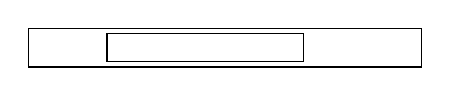
\begin{tikzpicture}

\draw (0,-2pt) rectangle (5,12pt);
\draw (1,0pt) rectangle (3.5,10pt);

\end{tikzpicture}

\caption{An impossible set of minimal windows: one window cannot be contained in another.}
\end{subfigure}

\caption{Visualizing the minimal windows of an episode.}
\label{fig:minimal-windows-chains}
\end{figure}
\fi


\section{Finding all minimal windows of parallel episodes}
\label{sec:rec-par-mwi}

\begin{algorithm}

\caption{Finding all of the minimal windows of a collection $ \mathcal{C} $ of parallel episodes in a sequence $ \boldsymbol{s} $. \\
Input: A collection $ \mathcal{C} $ of parallel episodes, an event sequence $ \boldsymbol{s} = (s, T_s, T_e) $, a window width $ \rho $, and a frequency threshold \textit{min\_fr}. \\
Output: All episodes in $ \mathcal{C} $, along with all minimal windows of each episode (including overlapping windows).}

\begin{algorithmic}[1]

\LineComment{Initialization}
\ForAll{event types $ A $}
    \State $ Q(A) \gets \text{empty queue} $
\EndFor
\ForAll{$ \alpha $ in $ \mathcal{C} $}
    \ForAll{$ A $ in $ \alpha $}
        \State $ \text{consider\_max}(\alpha, A) \gets 0 $
        \State $ \text{num\_needed}(\alpha, A) \gets \text{number of elements of type $ A $ in $ \alpha $} $
        \State $ \text{contains}(A) \gets \text{contains}(A) \cup \{ \alpha \} $
    \EndFor
\EndFor

\LineComment{Recognition}
\For{$ \text{start} \gets T_s - \rho + 1 $ to $ T_e - 1 $} % TODO check if starting at correct position
    \LineComment{Drop out old events from the window}
    \ForAll{events $ (A, t) $ in $ s $ such that $ t = \text{start} - 1 $}
        \State $ Q(A) \text{.pop}() $
    \EndFor

    \LineComment{Bring in new events to the window}
    \ForAll{events $ (A, t) $ in $ s $ such that $ t = \text{start} + \rho - 1 $}
        \State $ Q[A] \text{.push}(t) $ \label{alglin:rec-par-mwi:push-timestamp}
        \ForAll{$ \alpha $ in $ \text{contains}(A) $}
            \State $ \text{consider\_max}(\alpha, A) \gets \text{consider\_max}(\alpha, A) + 1 $
            \If{$ \forall A $ in $ \alpha : \min(| Q(A) |, \text{consider\_max}(\alpha, A)) \geq \text{num\_needed}(\alpha, A) $ } \label{alglin:rec-par-mwi:check-min-window-satisfied}
                \LineComment{Minimal window found; determine the start}
                \State $ \text{window\_start} \gets $ \label{alglin:rec-par-mwi:find-window-start}
                \State \hspace{\algorithmicindent} $ \min\{ t \mid A $ in $ \alpha \wedge t = Q(A)[| Q(A) | - \text{num\_needed}(\alpha, A) + 1] \} $
                \ForAll{$ A $ in $ \alpha $}
                    $ q \gets Q(A) $
                    \If{$ \text{window\_start} = q[| q | - \text{num\_needed}(\alpha, A)) + 1] $}
                        \State $ \text{consider\_max}(\alpha, A) \gets \text{num\_needed}(\alpha, A) - 1 $
                    \EndIf
                \EndFor
                \State append $ [\text{window\_start}, \text{start} + \rho) $ to $ \alpha \text{.minimal\_windows} $
            \EndIf
        \EndFor
    \EndFor
\EndFor

\end{algorithmic}

\label{alg:rec-par-mwi}
\end{algorithm}

Finding the minimal windows of parallel episodes is slightly more complex than determining their fixed-window frequency.

Thanks to the requirement that all minimal windows have a width of at most $ \rho $, we can keep using a sliding window of fixed width, just like the algorithms for the fixed-window frequency. Then only the part of the sequence included in the sliding window needs to be considered at any time, and any minimal window we find will be a subwindow of the current sliding window. We'll still be scanning the front of the sliding window for new events as before. Now, when a new event $ (A, t) $ comes in, we need to answer the following questions regarding episodes $ \alpha $ containing $ A $:
\begin{enumerate}
\item With this new event in the window, is there a minimal window $ [a, \text{start} + \rho) $ of $ \alpha $ which ends at the front of the current sliding window?
\item If so, where does the minimal window start: what is $ a $?
\end{enumerate}

Since minimal windows will often be smaller than the fixed-width sliding window, a previously recognized minimal window may still be within the sliding window several timestamps after it has been recognized. We need some way of excluding that previous minimal window from consideration, on a per-episode basis. Also, we need to be able to find the start of a new minimal window efficiently. It should be clear, then, that we need to keep more information than we did in algorithm~\ref{alg:rec-par-fwi}, where we just kept the number of events of each type currently in the sliding window, and for each episode, those event types for which there are enough events in the window to satisfy an occurrence anywhere in the sliding window.

Any newly discovered minimal window has to start \emph{after} the start of the previous one, because:
\begin{enumerate}
\item we already know it ends after the start of the previous one, since the sliding window has advanced, and
\item one minimal window of $ \alpha $ cannot be a subwindow of another.
\end{enumerate}

So, given the previous minimal window $ [a, b) $, all of the events that cannot contribute to a new minimal window are those with a timestamp $ t \leq a $. All those with $ t > a $ \emph{can} contribute.

Algorithm~\ref{alg:rec-par-mwi} keeps a queue for each event type $ A $, which contains the timestamps of the events of type $ A $ currently in the sliding window. The queues are referred to by $ Q $ in the pseudocode. When a new event $ (A, t) $ comes in, $ t $ is pushed onto $ Q(A) $ (line~\ref{alglin:rec-par-mwi:push-timestamp}). Then, for each episode $ \alpha $ containing $ A $, it is determined whether we have a new minimal window, by testing for each event type $ A $ in $ \alpha $ whether $ Q(A) $ contains enough events, excluding the events at the start of the most recently found minimal window (line~\ref{alglin:rec-par-mwi:check-min-window-satisfied}). The exclusion of these events is realized by \textbf{consider\_max}.

If we have determined that there are enough events in consideration to form a new minimal window, then the queues allow us to find the start of the window (line~\ref{alglin:rec-par-mwi:find-window-start}). If $ \alpha $ contains $ n $ nodes of type $ A $, then we look at the $ n $-th most recently added timestamp to $ Q(A) $. The earliest such timestamp for all event types in $ \alpha $ is the start of the minimal window.

% TODO explain the preceding a bit better maybe

[TODO add example figure]

\iffalse
\begin{figure}
\centering

\begin{tikzpicture}

\sequencetickmarks{7}{0}{0}
\sequenceeventtypes{0}{1em}{1}{1/a,2/b,3/a,4/b,5/c,6/b,7/a}

\windowthingy{(0,-5pt)}{2}
\windowthingy{(0.5,-10pt)}{2}
\windowthingy{(1,-5pt)}{2}
\windowthingy{(2.5,-5pt)}{2}

\end{tikzpicture}

\caption{All of the minimal windows of $ \{ a, b \} $ in the sequence.}
\label{fig:rec-par-mwi-example}
\end{figure}
\fi

\subsection{Notes on the implementation}

We need random access into the queues in order to find the start of a minimal window (line~\ref{alglin:rec-par-mwi:find-window-start}). The queues should therefore be implemented with a circular buffer.


\section{Finding all minimal windows of serial episodes}
\label{sec:rec-ser-mwi}

\begin{algorithm}

\caption{Recognizing serial episodes using the minimal window frequency measure. \\
Input: An array of serial episodes $ \mathcal{C} $, an event sequence $ \boldsymbol{s} = (s, T_s, T_e) $, a window width $ \rho $, and a frequency threshold \textit{min\_fr}. \\
Ouptut: All episodes in $ \mathcal{C} $, along with all minimal windows of each episode (including overlapping windows).
}

\begin{algorithmic}[1]

\ForAll{$ \alpha \in \mathcal{C} $} \Comment{Initialization}
    \For{$ i \leftarrow 1 $ to $ | \alpha | $}
        \State{$ \alpha \text{.initialized}[i] \leftarrow \text{\textit{uninitialized}} $}
        \State{$ \text{waits}(\alpha[i]) \leftarrow \emptyset $}
    \EndFor
\EndFor

\ForAll{$ \alpha \in \mathcal{C} $}
    \State{$ \text{waits}(\alpha[1]) \leftarrow \text{waits}(\alpha[1]) \cup \left\{ \left( \alpha, 1 \right) \right\} $} \label{alglin:rec-ser-mwi:fill-waits-init}
    \State{$ \alpha \text{.minimal\_windows} \gets \emptyset $}
\EndFor

\For{$ t \leftarrow T_s - \rho $ to $ T_s - 1 $} $ \text{begins\_at}(t) \leftarrow \emptyset $
\EndFor
\For{$ \text{start} \leftarrow T_s - \rho + 1 $ to $ T_e $} \label{alglin:rec-ser-mwi:iterate-sequence} \Comment{Recognition}
    \State{$ \text{begins\_at}(\text{start} + \rho - 1) \leftarrow \emptyset $}
    \State{$ \text{transitions} \leftarrow \emptyset $}
    \ForAll{$ (\alpha, l) \in \text{begins\_at}(\text{start} - 1) $} \label{alglin:rec-ser-mwi:cleanup-for}
        \If{$ l < | \alpha | $} \label{alglin:rec-ser-mwi:cleanup-iteration-begin}
            \State{$ \text{waits}(\alpha [l + 1]) \leftarrow \text{waits}(\alpha [l + 1]) \setminus \{ ( \alpha, l + 1 ) \} $}
        \EndIf
        \State{$ \alpha \text{.initialized}[l] \leftarrow \text{\textit{uninitialized}} $} \label{alglin:rec-ser-mwi:cleanup-iteration-end}
    \EndFor
    \ForAll{events $ (A, t) $ in $ s $ such that $ t = \text{start} + \rho - 1 $} \label{alglin:rec-ser-mwi:iterate-new-events}
        \ForAll{$ ( \alpha, j) \in \text{waits}(A) $}
            \If{$ j = 1 $} \label{alglin:rec-ser-mwi:add-to-transitions}
                \State{$ \text{transitions} \leftarrow \text{transitions} \cup \{ ( \alpha, 1, \text{start} + \rho - 1 ) \} $}
            \Else
                \State{$ \text{transitions} \leftarrow \text{transitions} \cup \{ \alpha, j, \alpha \text{.initialized} [j - 1] \} $}
                \State{$ \text{begins\_at}( \alpha \text{.initialized}[j - 1] ) \leftarrow $ \label{alglin:rec-ser-mwi:cleanup-old-states}
                \State \hspace{\algorithmicindent} $ \text{begins\_at}( \alpha \text{.initialized}[j - 1] ) \setminus \{ ( \alpha, j - 1 ) \} $}
                \State{$ \alpha \text{.initialized} [j - 1] \leftarrow \text{\textit{uninitialized}} $}
                \State{$ \text{waits}(A) \leftarrow \text{waits}(A) \setminus \{ ( \alpha, j ) \} $}
            \EndIf
        \EndFor
    \EndFor
    \ForAll{$ ( \alpha, j, t ) \in \text{transitions} $}
        \If{$ \alpha \text{.initialized}[j] \neq \text{\textit{uninitialized}} $} \label{alglin:rec-ser-mwi:added-line-1} \label{alglin:rec-ser-mwi:transition-begin}
            \State $ \text{begins\_at}(\alpha \text{.initialized}[j]) \gets \text{begins\_at}(\alpha \text{.initialized}[j]) \setminus \{ (\alpha, j) \} $ \label{alglin:rec-ser-mwi:added-line-2}
        \EndIf
        \State{$ \alpha \text{.initialized} [j] \leftarrow t $}
        \State{$ \text{begins\_at}(t) \leftarrow \text{begins\_at}(t) \cup \{ ( \alpha, j ) \} $}
        \If{$ j = | \alpha | $}
            \State $ \alpha \text{.minimal\_windows} \gets $
            \State \hspace{\algorithmicindent} $ \alpha \text{.minimal\_windows} \cup \{ [\alpha \text{.initialized}[j], \text{start} + \rho) \} $
        \Else
            \State{$ \text{waits}(\alpha [j + 1]) \leftarrow \text{waits}(\alpha [j + 1]) \cup \{ (\alpha, j + 1) \} $} \label{alglin:rec-ser-mwi:transition-end}
        \EndIf
    \EndFor
\EndFor

\end{algorithmic}

\label{alg:rec-ser-mwi}
\end{algorithm}

While finding the minimal windows of parallel episodes was slightly more complicated than finding their fixed-window frequency, finding the minimal windows of serial episodes is actuallly simpler than finding their fixed-window frequency, and can be accomplished with small changes to algorithm~\ref{alg:rec-ser-fwi}.

Algorithm~\ref{alg:rec-ser-mwi} accomplishes recognition of serial episodes using the minimal window frequency measure.

Once an automaton instance for an episode $ \alpha $ has reached state $ | \alpha | $, we know immediately where a minimal window starts and ends---it starts at the point where the automaton was initialized, and ends at the front of the current sliding window: $ \boldsymbol{s}[\alpha \text{.initialized}[| \alpha |], \allowbreak \text{start} + \rho) $. So, in contrast to the situation for fixed windows, now there is no second phase in which to keep track of the displacement of the sliding window, and therefore the \emph{in\_window} variable isn't needed.

In this adaptation, old events are removed before new ones are processed, because the situation explained in footnote~\ref{footnote:false-recognition} on page~\pageref{footnote:false-recognition} would become a problem when the frequency isn't determined by the displacement of the sliding window anymore.

% As we discussed in footnote~\ref{footnote:false-recognition}, the recognition algorithms for fixed windows recognize occurrences of widths up to $ \rho + 1 $ because new events are processed before old events are dropped. There, that's not a problem since the recognition of such an  will result in a sliding window displacement of $ 0 $, such that the frequency count of a falsely recognized episode isn't affected. Here, that would not work though, because we don't determine frequency based on sliding window displacement anymore. Therefore we remove old events before letting new events enter the sliding window.

Figure~\ref{fig:parallel-minimal-recognition} shows how the algorithm finds the minimal windows of an episode $ \{ a, a, b \} $ in an example sequence.

\begin{figure}
\centering

\begin{tikzpicture}

\def\slidingwindowheight{0.5}
\def\interdotdistance{0.6}

\newcommand\letteratposition[1]
{\ifnum#1=2a\else\ifnum#1=3b\else\ifnum#1=5a\else\ifnum#1=7a\else0\fi\fi\fi\fi}

\newcommand\slidingwindowthingy[2]
{
    \foreach \i [evaluate=\i as \x using \i * \interdotdistance] in {0,...,7}
    {
        \ifnum\pdfstrcmp{\letteratposition{\i}}{0}=0
            \fill (\x,#1) circle [color=black,radius=2pt] node (n#2-\i) {};
        \else
            \draw (\x,#1) node [enoughdamnvspace] (n#2-\i) {$ \letteratposition{\i} $};
        \fi
    }

    \node (dr#2) [right=7pt of n#2-7] {$ \cdots $};
}

\slidingwindowthingy{0}{0}
\draw (-0.5*\interdotdistance,-0.5*\slidingwindowheight) -- ++(2*\interdotdistance,0) -- ++(0,\slidingwindowheight) -- ++(-2*\interdotdistance,0);
\node (Qa) [right=1.5em of dr0,rotate=90,anchor=west,xshift=0.6cm] {$ Q(a) $};
\node (Qb) [right=4em of dr0,rotate=90,anchor=west,xshift=0.6cm] {$ Q(b) $};
\node (maxconsidera) [right=6em of dr0,rotate=90,anchor=west,xshift=0.6cm] {$ \text{max\_consider}(\alpha, a) $};
\node (maxconsiderb) [right=7.5em of dr0,rotate=90,anchor=west,xshift=0.6cm] {$ \text{max\_consider}(\alpha, b) $};

\node at (Qa |- dr0) {$ \langle \; \rangle $};
\node at (Qb |- dr0) {$ \langle \; \rangle $};
\node at (maxconsidera |- dr0) {$ 0 $};
\node at (maxconsiderb |- dr0) {$ 0 $};

\node at (n0-0 |- {(0,0.75)}) {\footnotesize $ 1 $};
\node at (n0-2 |- {(0,0.75)}) {\footnotesize $ 3 $};
\node at (n0-4 |- {(0,0.75)}) {\footnotesize $ 5 $};
\node at (n0-6 |- {(0,0.75)}) {\footnotesize $ 7 $};

\slidingwindowthingy{-1}{1}
\draw (-0.5*\interdotdistance,-1-0.5*\slidingwindowheight) -- ++(3*\interdotdistance,0) -- ++(0,\slidingwindowheight) -- ++(-3*\interdotdistance,0);

\node at (Qa |- dr1) {$ \langle 3 \rangle $};
\node at (Qb |- dr1) {$ \langle \; \rangle $};
\node at (maxconsidera |- dr1) {$ 1 $};
\node at (maxconsiderb |- dr1) {$ 0 $};

\slidingwindowthingy{-2}{2}
\draw (-0.5*\interdotdistance,-2-0.5*\slidingwindowheight) -- ++(4*\interdotdistance,0) -- ++(0,\slidingwindowheight) -- ++(-4*\interdotdistance,0);

\node at (Qa |- dr2) {$ \langle 3 \rangle $};
\node at (Qb |- dr2) {$ \langle 4 \rangle $};
\node at (maxconsidera |- dr2) {$ 1 $};
\node at (maxconsiderb |- dr2) {$ 1 $};

\slidingwindowthingy{-3}{3}
\draw (-0.5*\interdotdistance,-3-0.5*\slidingwindowheight) rectangle ++(6*\interdotdistance,\slidingwindowheight);

\node at (Qa |- dr3) {$ \langle 3, 6 \rangle $};
\node at (Qb |- dr3) {$ \langle 4 \rangle $};
\node at (maxconsidera |- dr3) {$ 2 $};
\node at (maxconsiderb |- dr3) {$ 1 $};

\node [right=9em of dr3,align=left] {enough events in window\\and in consideration;\\minimal window found};

\draw ({(1.5*\interdotdistance,0)} |- n3-2.south) -- ++(0,-6pt) -- node (numwindowsindicator) [near start,below right,align=left] {determine minimal window \\ using \emph{num\_needed}, $ Q $, and \emph{start}} ++(4*\interdotdistance,0) -- ++(0,6pt);

\slidingwindowthingy{-5.25}{4}
\draw (0.5*\interdotdistance,-5.25-0.5*\slidingwindowheight) rectangle ++(6*\interdotdistance,\slidingwindowheight);

\node at (Qa |- dr4) {$ \langle 3, 6 \rangle $};
\node at (Qb |- dr4) {$ \langle 4 \rangle $};
\node at (maxconsidera |- dr4) {$ 1 $};
\node at (maxconsiderb |- dr4) {$ 1 $};

\node [right=9em of dr4,align=left] {previous occurrence still in\\window, but first $ a $ out of \\ consideration};

\slidingwindowthingy{-7}{5}
\draw (1.5*\interdotdistance,-7-0.5*\slidingwindowheight) rectangle ++(6*\interdotdistance,\slidingwindowheight);

\node at (Qa |- dr5) {$ \langle 3, 6, 8 \rangle $};
\node at (Qb |- dr5) {$ \langle 4 \rangle $};
\node at (maxconsidera |- dr5) {$ 2 $};
\node at (maxconsiderb |- dr5) {$ 1 $};

\node [right=9em of dr5,align=left] {new $ a $ entered; \\ another minimal window \\ found};

\draw ({(2.5*\interdotdistance,0)} |- n5-3.south) -- ++(0,-6pt) -- ++(5*\interdotdistance,0) -- ++(0,6pt);

\slidingwindowthingy{-8.5}{6}
\draw (7.5*\interdotdistance,-8.5-0.5*\slidingwindowheight) -- ++(-5*\interdotdistance,0) -- ++(0,\slidingwindowheight) -- ++(5*\interdotdistance,0);

\node at (Qa |- dr6) {$ \langle 6, 8 \rangle $};
\node at (Qb |- dr6) {$ \langle 4 \rangle $};
\node at (maxconsidera |- dr6) {$ 2 $};
\node at (maxconsiderb |- dr6) {$ 0 $};

\end{tikzpicture}

\caption{Recognition of parallel episode $ \alpha = \{ a, a, b \} $, finding its minimal windows in the sequence. Black dots are timestamps that don't contain $ a $ or $ b $.}
\label{fig:parallel-minimal-recognition}
\end{figure}

\section{Determining the weighted-window frequency}

\begin{algorithm}

\caption{Computing the weighted frequency of an episode in a sequence.\\
Input: A list of minimal windows $ V = \langle \, [a_1, b_1), \, \ldots, \, [a_n, b_n) \rangle $ of episode $ \alpha $.\\
Output: $ fr_w(\alpha) $
}

\begin{algorithmic}[1]

\State $ j \gets 1 $
\ForAll {$ [a_i, b_i) \in V $} \label{alglin:wwi:begin-next-disjoint-window}
    \While {$ j \leq n \wedge b_i > a_j $}
        \State $ j \gets j + 1 $
    \EndWhile
    \State $ d_i \gets j $ \label{alglin:wwi:end-next-disjoint-window}
\EndFor
\State $ c_{n + 1} \gets 0 $ \label{alglin:wwi:begin-wwi-calculation}
\For {$ i \gets n $ down to $ 1 $}
    \State $ c_i \gets \max((b_i - a_i)^{-1} + c_{d_i}, \; c_{i+1}) $ \label{alglin:wwi:end-wwi-calculation}
\EndFor
\State output $ c_1 $

\end{algorithmic}

\label{alg:wwi}
\end{algorithm}

For the weighted-window frequency, selecting the non-overlapping minimal windows such that total weight is maximal, is a bit more involved than selecting the largest possible number of non-overlapping minimal windows for the disjoint-window frequency (section~\ref{sec:disjoint-window-frequency}).

In algorithm~\ref{alg:wwi} (from~\cite{cule2014marbles}), lines~\ref{alglin:wwi:begin-next-disjoint-window} through~\ref{alglin:wwi:end-next-disjoint-window}, for each minimal window $ [a_i, b_i) $ the \emph{next} window disjoint from $ [a, b) $ is determined, and referred to by $ d_i $. More precisely, $ d_i $ refers to the window $ [a_j, b_j) $ with the smallest $ a_j $ such that $ a_j \geq b_i $.

Then, in lines~\ref{alglin:wwi:begin-wwi-calculation} through~\ref{alglin:wwi:end-wwi-calculation}, the weighted-window frequency is determined through a backwards pass over the minimal windows. Each $ c_i $ is the optimal choice of windows $ i $ through $ n $. If all $ c_j $ with $ j > i $ are known, then $ c_i $ can be calculated as
\begin{align*}
c_i = \max((b_i - a_i)^{-1} + c_{d_i}, \; c_{i+1})
\end{align*}
where the leftmost argument to $ \max $ represents selecting window $ i $, and therefore ``unselecting'' all earlier selected windows that overlap with window $ i $, and the rightmost argument to $ \max $ represents not selecting window $ i $ and continuing with all previously selected windows.

In this way, the $ d_i $ essentially allow us to \emph{backtrack} to undo earlier choices in favour of a better one.



\section{Removing episodes which have been found infrequent}
\label{sec:maintain-blocks}

\begin{algorithm}

\caption{Removing infrequent episodes from a collection of candidates $ \mathcal{C} $ for which \emph{freq\_count} is known. \\
Input: A sorted array of candidates $ \mathcal{C} $, including their \emph{block\_start} values, and their \emph{freq\_count} values with respect to some sequence, and a minimum frequency threshold \emph{min\_fr}. \\
Output: A sorted array $ \mathcal{F} $ of those episodes in $ \mathcal{C} $ which are frequent, along with consistent \emph{block\_start} values.
}

\begin{algorithmic}[1]

\State $ \text{new\_block\_start} \gets 1 $
\State $ \mathcal{F} \gets \text{empty array} $
\State $ \mathcal{F} \text{.block\_start} \gets \text{empty array} $
\For{$ i \gets 1 $; $ i \leq | \mathcal{C} | $; $ i \gets i + 1 $}
    \If{$ \mathcal{C} \text{.block\_start}[i] = i $} \label{alglin:remove-infrequent-episodes:different-block-test}
        \LineComment{Encountered new block in $ \mathcal{C} $}
        \State $ \text{new\_block\_start} \gets | \mathcal{F} | $
    \EndIf
    \If{$ \alpha \text{.freq\_count} < \text{min\_fr} $}
        \LineComment{Episode infrequent; discard}
        \State continue with next $ i $
    \EndIf
    \State append $ \alpha $ to $ \mathcal{F} $
    \State $ \mathcal{F} \text{.block\_start}[ | \mathcal{F} | ] \gets \text{new\_block\_start} $
\EndFor
\State output $ \mathcal{F} $

\end{algorithmic}

\label{alg:remove-infrequent-episodes}
\end{algorithm}

At first sight, it seems a trivial task to discard episodes from a list of candidates which have turned out to be infrequent. But one thing needs to be taken into consideration, namely the auxiliary \emph{block\_start} variables, used in the candidate generation algorithm (section~\ref{sec:cand-gen}). Each episode $ \alpha $ has such a \emph{block\_start} value, which denotes the array index of the first episode in the list with which it shares the first $ | \alpha | - 1 $ elements in the episode's array representation. If we remove episodes without further consideration, these indices will be invalidated. They should not be invalidated, however, since the next round of the candidate generation step relies on them. Hence we need to keep track of the blocks while constructing the list of frequent episodes. Algorithm~\ref{alg:remove-infrequent-episodes} achieves this.

The algorithm stores the frequent episodes in a new data structure $ \mathcal{F} $. While iterating over the episodes in order, the array index of the new block start is kept in \emph{new\_block\_start}. If for an index $ i $, $ \mathcal{C}. \text{block\_start}[i] = i $, we know that a new block started at position $ i $ in $ \mathcal{C} $, and so \emph{new\_block\_start} gets updated in order to start a new block in $ \mathcal{F} $ as well.



\section{Finding association rules from frequent episodes: high-level algorithm}

\begin{algorithm}

\caption{Finding confident association rules composed of frequent episodes.\\
Input: A window width $ \rho $, a frequency/confidence measure $ \Psi $, a frequency threshold \emph{min\_fr}, and a confidence threshold \emph{min\_conf}.\\
Output: $ \{ (\alpha \Rightarrow \beta, c(\alpha \Rightarrow \beta)) \mid \beta \subset \alpha \wedge fr(\beta) \geq \text{min\_fr} \wedge c(\alpha \Rightarrow \beta) \geq \text{min\_conf} \} $
}

\begin{algorithmic}[1]

\LineComment{Find frequent episodes (algorithm~\ref{alg:episodes-top-level})}
\State compute $ \mathcal{F}(\boldsymbol{s}, \rho, \text{min\_fr}) $
\LineComment{Generate rules}
\ForAll{$ \beta \in \mathcal{F}(\boldsymbol{s}, \rho, \text{min\_fr}) $}
    \ForAll{$ \alpha \subset \beta $}
        \If{$ c_\Psi(\alpha \Rightarrow \beta) \geq \text{min\_conf} $} \label{alglin:association-rules-top-level:compute-confidence}
            \State output $ \alpha \Rightarrow \beta $ and $ c_\Psi(\alpha \Rightarrow \beta) $
        \EndIf
    \EndFor
\EndFor

\end{algorithmic}

\label{alg:association-rules-top-level}
\end{algorithm}

Now that we have described the full solution for mining frequent episodes, let's turn to association rules. Algorithm~\ref{alg:association-rules-top-level} (adapted from \citep{mannila1997discovery}) shows the high-level procedure for generating confident association rules after mining frequent episodes.

On line~\ref{alglin:association-rules-top-level:compute-confidence}, to decide whether a newly constructed association rule $ \alpha \Rightarrow \beta $ is confident, its confidence value must be computed. For the fixed-window confidence this is trivial: given the frequency of both episodes, compute
\begin{align*}
c_f(\alpha \Rightarrow \beta) = \frac{fr(\beta)}{fr(\alpha)}
\end{align*}

For the minimal-window confidence and the weighted-window confidence, we use the minimal windows found while mining frequent episodes; in algorithms~\ref{alg:minimal-window-confidence} (section~\ref{sec:minimal-window-confidence}) and \ref{alg:weighted-window-confidence} (section~\ref{sec:weighted-window-confidence}), respectively.

\section{Determining the minimal-window confidence}
\label{sec:minimal-window-confidence}

\begin{algorithm}

\caption{Computing the minimal-window confidence of an association rule $ \alpha \Rightarrow \beta $.\\
Input: List of minimal windows $ V = \langle [a_1, b_1), \ldots, [a_n, b_n) \rangle $ of episode $ \alpha $, list of minimal windows $ W = \langle [p_1, q_1), \ldots, [p_m, q_m) \rangle $ of episode $ \beta $.\\
Output: $ c_m(\alpha \Rightarrow \beta) $
}

\begin{algorithmic}[1]

\State $ u \gets 0 $
\State $ j \gets 1 $
\ForAll{$ i \gets 1 $ to $ n $} \label{alglin:minimal-window-confidence:for}
    \While{$ j \leq m \wedge q_j < b_i $} \label{alglin:minimal-window-confidence:while}
        \State $ j \gets j + 1 $
    \EndWhile
    \If{$ j \leq m \wedge p_j \leq a_i $} $ u \gets u + 1 $ \label{alglin:minimal-window-confidence:increment}
    \EndIf
\EndFor
\State output $ u / n $

\end{algorithmic}

\label{alg:minimal-window-confidence}
\end{algorithm}

Algorithm~\ref{alg:minimal-window-confidence}, adapted from~\citep{cule2014marbles}, computes the minimal-window confidence of an association rule $ \alpha \Rightarrow \beta $, given a list $ V $ of the minimal windows of $ \alpha $ and a list $ W $ of the minimal windows of $ \beta $, both lists ordered by the timestamps that define the windows. Both lists are iterated once, simultaneously.

For each minimal window $ [a_i, b_i) $ of $ \alpha $, we need to determine if there exists a minimal window $ [p_j, q_j) \supset [a_i, b_i) $ of $ \beta $. If so, $ ext_m([a, b), \alpha, \beta) = 1 $. For each window in $ V $, (line~\ref{alglin:minimal-window-confidence:for}), $ W $ is traversed (line~\ref{alglin:minimal-window-confidence:while}) until for a minimal window $ [p_j, q_j) $ in $ W $, a comparison of the end timestamps of both windows determine that $ q_j \geq b_i $. Then the start timestamps are compared (line~\ref{alglin:minimal-window-confidence:increment}): if $ p_j \leq a_i $, then we know that $ [p_j, q_j) \supset [a_i, b_i) $. Note that $ W $ does not need to be traversed from the beginning for each window in $ V $, since both lists are ordered by timestamp.

If it turns out that $ ext_m([a, b), \alpha, \beta) = 1 $ for a minimal window $ [a, b) $, then this gets registered by incrementing variable $ u $ (line~\ref{alglin:minimal-window-confidence:increment}).

\iffalse
\begin{figure}
\centering

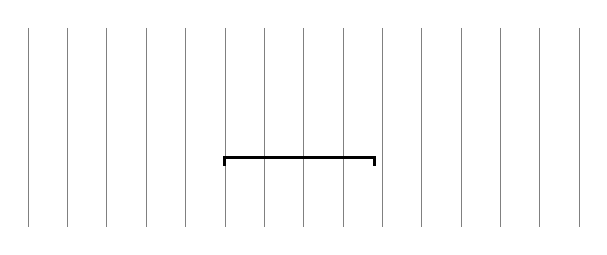
\begin{tikzpicture}

\sequencetickmarks{15}{0}{0}

\foreach \x in {0,0.5,...,7}
    \draw [gray,ultra thin] (\x,2) -- (\x,-15pt);

\draw [very thick] (2.5,10pt) ++(0,-3pt) -- ++(0,3pt) -- ++(1.9,0) -- +(0,-3pt);
\windowthingy{(1,-5pt)}{5}
\windowthingy{(2,-10pt)}{6}

\end{tikzpicture}

\caption{Finding a minimal window of $ \beta $ that contains a given minimal window of $ \alpha $ (drawn above the sequence tick marks in bold).}
\label{fig:minimal-window-confidence}
\end{figure}
\fi

\subsection{Correcting the original algorithm presented in~\cite{cule2014marbles}}

In~\citep{cule2014marbles}, there is a small mistake in algorithm~\ref{alg:minimal-window-confidence} (algorithm~1 in~\citep{cule2014marbles}), regarding the comparison of the end timestamps of two windows. In the condition for the \emph{while}-statement, $ W $ is traversed until a window with an end timestamp \emph{strictly} greater than the end timstamp of the window in $ V $ currently being considered. However, one window can be a subwindow of another if their end timestamps are equal. If implemented as written in~\cite{cule2014marbles}, then a minimal window in $ W $ could be skipped erroneously.



\section{Determining the weighted-window confidence}
\label{sec:weighted-window-confidence}

\begin{algorithm}

\caption{Computing the weighted-window confidence of an association rule $ \alpha \Rightarrow \beta $.\\
Input: A list of the minimal windows $ V = \langle [a_1, b_1), \ldots, [a_n, b_n) \rangle $ of episode $ \alpha $, and a list of the minimal windows $ W = \langle [p_1, q_1), \ldots, [p_m, q_m) \rangle $ of episode $ \beta $.\\
Output: $ c_w(\alpha \Rightarrow \beta) $
}

\begin{algorithmic}[1]

\State $ c \gets 0 $
\State $ i \gets 1 $
\For{$ k \gets 1 $ to $ n $}
    \While{$ i \leq m \wedge p_i < b_k $}
        \State $ i \gets i + 1 $
    \EndWhile
    \State $ j \gets i $
    \State $ l \gets +\infty $
    \While{$ j \leq m \wedge p_j \leq a_k $} \label{alglin:weighted-window-confidence:find-smallest-while}
        \If{$ q_j - p_j \leq l $}
            \State $ l \gets q_j - p_j $
            \State $ i \gets j $
        \EndIf
        \State $ j \gets j + 1 $
    \EndWhile
    \If{$ l \in \mathbb{N} $}
        \State $ c \gets c + (b_i - a_i) / l $
    \EndIf
\EndFor
\State output $ c / n $

\end{algorithmic}

\label{alg:weighted-window-confidence}
\end{algorithm}

The calculation of the weighted-window confidence of an association rule can be done in a similar vein as the minimal-window confidence (section~\ref{sec:minimal-window-confidence}). The main difference is that now, not only do we have to determine whether or not there exists a window in $ W $ contains a given $ [a_k, b_k) \in V $; if such windows exist, we have to find the \emph{smallest} one in order to compute $ ext_w([a_i, b_i), \alpha, \beta) $, given definition~\ref{def:weighted-extensibility}.

This is what happens in the second \emph{while}-loop in algorithm~\ref{alg:weighted-window-confidence} (line~\ref{alglin:weighted-window-confidence:find-smallest-while}, algorithm adapted from~\cite{cule2014marbles}). After the first minimal window $ [p_i, q_i) \supset [a_k, b_k) $ has been found, all subsequent windows $ [p_j, q_j) \supset [a_k, b_k) $ are checked for their length. The index $ j $ for which the weight $ (q_j - p_j)^{-1} $ is maximal, is stored in $ i $, and the corresponding window contributes towards the weighted-window confidence.

\subsection{Correcting the algorithm presented in~\citep{cule2014marbles}}

Algorithm 3 from~\citep{cule2014marbles}---which algorithm~\ref{alg:weighted-window-confidence} was based on---does not account for the possibility that there is no minimal window of $ \beta $ that contains the current minimal window of $ \alpha $. To that end, we update $ c $ only if at least one such window exists.

\section{Finding all subepisodes of a parallel episode}

While generating association rules in algorithm~\ref{alg:association-rules-top-level}, we need to consider all subepisodes $ \alpha $ of each frequent episode $ \beta $. For serial episodes, we take all possible combinations of leaving out nodes from the episode graph. Using this approach, the number of subepisodes to be considered is exponential This will sometimes produce equivalent episodes, namely when the same event type occurs multiple times. Take, for instance the episode $ a \to a $.

% TODO consider dropping this...
